\section{Evaluation}
\label{compare}

We carried out an extensive evaluation of \method.
We first analyse the three state of the art techniques for efficiency model computation in Section~\ref{eval-efficiency} and privacy leakage in Section~\ref{eval-leakage}, before summarizing the comparison Section~\ref{eval-summary}.
We then evaluate the proposed training methodology in Section~\ref{evalPh1} and Section~\ref{evalPh2} for Phase I and Phase II, respectively.
Finally, we compare \method~ against state of the art defence schemes in Section~\ref{eval-defences}.


\subsection{Evaluating Efficiency}
\label{eval-efficiency}

In this section, in the view of the memory-computation-energy efficiency requirements, we compare the three baseline algorithms (i.e., model compression, off-the-shelf architecture, and quantization).
%We then select an efficient design scheme for NNs that satisfies all our requirements.


\noindent\textbf{Memory Efficiency.} Off the shelf models are designed to specifically reduce the memory footprint.
For instance, the memory footprint of Squeezenet and MobileNet is 5MB and 14Mb compared to 250Mb of Alexnet and >500Mb of VGG architectures~\cite{DBLP:journals/corr/IandolaMAHDK16,conf/cvpr/SandlerHZZC18}.
Additionally, lowering the model precision from 64 or 32 bit floating point to binary precision results in a direct reduction of 64x or 32x in the overall memory footprint of the model.
However, in case of model compression the model parameters which are pruned are simply replaced by a value of "0".
Hence, storing even the "0" parameter takes up memory and does not necessarily decrease the overall memory footprint unless the hardware is optimized to skip the storage of all the zero values in the memory.
This requires additional logic to check for zero valued parameters in a dictionary.


\noindent\textbf{Computation Efficiency.} Design of efficient off-the-shelf architectures replaces the complex matrix-vector multiplications to smaller dimensions.
This reduces the overall number of parameters but it has been shown empirically\footnote{https://github.com/albanie/convnet-burden} that this does not necessarily reduce the number of multiply accumulate operations~\cite{article}.
In case of parameter pruning, achieving efficiency requires additional hardware optimization. Particularly, instead of actually computing the multiplications with "0" pruned values, the hardware optimization enables the user to skip the computation and replace the output by a "0" directly.
For quantized models with binarized parameters and activations the MACs can be replaced by binary XNOR operations, maxpool replaced by OR operation, while the activations can be replaced by checking the sign bit and hence reducing the FLOPS drastically~\cite{235489}.
This results in high computational efficiency and hence, faster inference.


\noindent\textbf{Energy Efficiency.} Energy efficiency does not vary much with reduction of number of parameters and data type, but the number of memory accesses play vital role~\cite{6757323}.
Specifically, for the case of off-the-shelf architectures, while computation efficiency improves, the energy efficiency is close to large scale state of the art models like AlexNet~\cite{DBLP:journals/corr/IandolaMAHDK16,8114708}.
Alternatively, for the case of model compression, energy efficiency can be marginally improved by additionally providing hardware optimization~\cite{journals/corr/YangCS16a,DBLP:journals/corr/HanMD15}.
For quantization, however, the energy efficiency is high as the memory access can be drastically reduced by increasing the throughput of data fetched from the memory.
Specifically, lowering the precision from 32 bit floating point to binary results in lowering the memory accesses and 32x improvement in energy consumption~\cite{NIPS2016_6573,rastegari2016xnornet}.
While some improvements are seen natively for quantized models (from replacing MACs with XNOR), higher benefits can be achieved via additional hardware optimization~\cite{Umuroglu2017FINNAF}.
The benchmarking of energy consumption for different optimization and architectures is well explored in the literature and out of scope of this work. We refer the readers to~\cite{8114708} for more details.

In summary, compared to different optimization techniques for NNs, the quantized architectures show significant benefits for different efficiency requirements over the other alternatives.




\subsection{Evaluating Privacy Leakage}
\label{eval-leakage}

In this section, we evaluate the information leakage through membership inference attacks for the three baseline algorithms considered.
This is the main contribution of our work where we evaluate the privacy leakage for different optimization and design algorithms for NNs.

\subsubsection{Model Compression}

We evaluate the privacy leakage on compressing a model by pruning the connections in the model.
Here, pruning is achieved by replacing some of the parameters with "0" value.
As described in the original paper~\cite{Han:2015:LBW:2969239.2969366,DBLP:journals/corr/HanPNMTECTD16}, pruning is followed by retraining the model to restore the model's original accuracy with the pruned connections.
We evaluate and validate the impact on membership privacy on compressing the model trained on two datasets: FashionMNIST and CIFAR10.

\textbf{Impact of Pruning Parameters.} On pruning the model, the model's test accuracy decreases but also lowers the membership inference accuracy (as seen for FashionMNIST in Figure~\ref{fig:prune}).
As the compression rate increases, the generalization error decreases (owing to a decrease in both train and test accuracy) with a decrease in membership accuracy to close to random guess.
This is expected as the parameters are responsible for memorizing the training data information~\cite{DBLP:journals/corr/abs-1812-00910,236216,10.1145/3133956.3134077} and pruning the parameters lowers the adversary's attack success.

\begin{figure}[!htb]
    \centering
    \begin{minipage}[b]{1\linewidth}
    \centering
    \subfigure[Impact of Model Pruning on Privacy]{
    \label{fig:prune}
    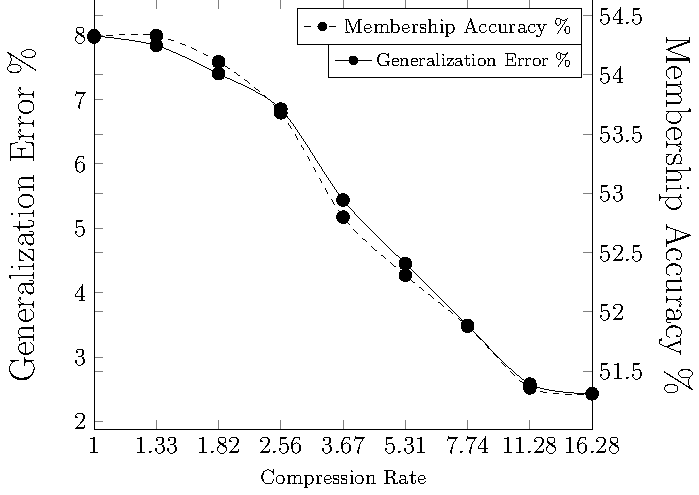
\includegraphics[width=0.7\linewidth]{figures/fmnist_prune.pdf}
    }
    \subfigure[Impact of Retraining on Privacy]{
    \label{fig:retrain}
    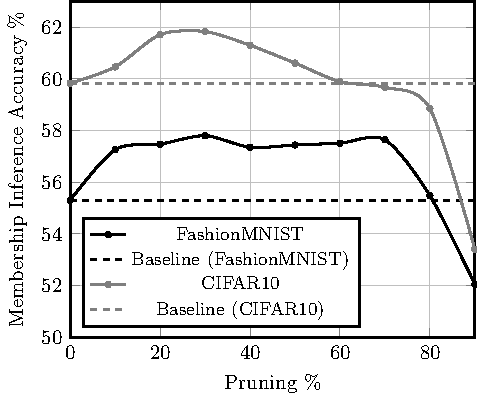
\includegraphics[width=0.7\columnwidth]{figures/retrain.pdf}
    }
    \subfigure[Mitigating Privacy Leakage via Weight Sharing]{
    \label{fig:wtsharing}
    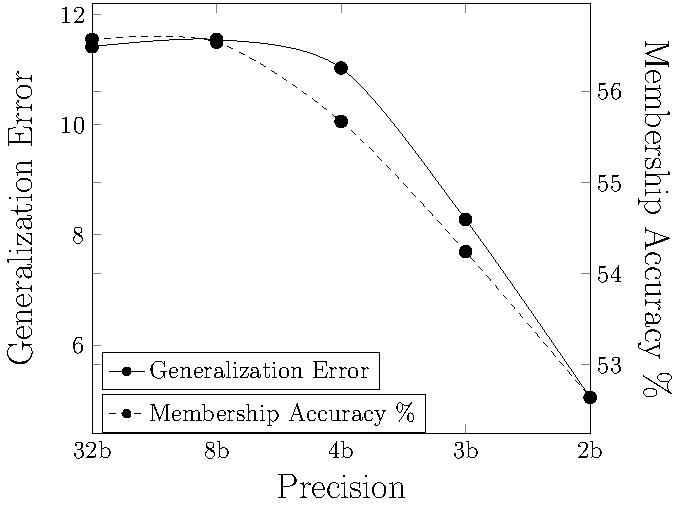
\includegraphics[width=0.7\linewidth]{figures/fmnist_wtsharing.pdf}
    }

    \end{minipage}
    \caption{Pruning the model lowers the membership inference leakage at the cost of accuracy. Retraining the pruned model to restore accuracy results in a higher membership privacy leakage compared to uncompressed baseline model. This additional leakage can be mitigated by weight sharing at the cost of accuracy.}
    \label{fig:NIAcause}
\end{figure}


\textbf{Impact of Retraining Pruned Model.} Interestingly, on retraining the pruned model, we observe that the membership inference accuracy is much higher than the original unpruned baseline model (Figure~\ref{fig:retrain}).
This indicates that model compression in turn increases the overall privacy leakage.
This can be attributed to the lower number of parameters forced to learn the same amount of information stored previously in the unpruned model with larger number of parameters.
In other words, the same amount of information is now captured by less number of parameters resulting in higher memorization of information per parameter.
As the model is compressed (pruned), the number of parameters decreases which results in increase in information per parameter. However, on aggressive pruning, the train and test accuracy also decreases resulting in a decrease in the information per parameter, which is empirically indicated by a decrease in membership inference accuracy at the end in Figure~\ref{fig:retrain}.

%To analyze the information stored per parameter, we first compute the model capacity as the mutual information of a trained network between the true label $Y$ and the predicted label $Y_{\theta}$ for a random input $X$ as derived in~\cite{45932,cap}.
%Here, model's information $I(Y;Y_{\theta}|X) = $
%\begin{equation}
%\footnotesize
%N_{train}\left(1 - (r_{train}log_2(\frac{1}{r_{train}}) + (1-r_{train})log_2(\frac{1}{1-r_{train}}))\right)
%\end{equation}
%where $r_{train}$ is the classification train accuracy for all the $N_{train}$ samples in the training data.
%For $r_{train} = 1$, the model completely memorizes all random samples as the information stored equals the number of samples $N_{train}$, while for $r_{train}=0.5$, the training accuracy 0.
%We divide the above equation by the model's total number of parameters $N_{param}$ to get the per parameter information stored as
%\begin{equation}
%I_p(Y;Y_{\theta}|X) = \frac{I(Y;Y_{\theta}|X)}{N_{param}}
%\end{equation}

In summary, model compression results in a higher membership privacy leakage compared to the baseline uncompressed model making it a poor candidate for applications with sensitive data.

\textbf{Mitigating the Privacy Risks in Pruned Models.} We describe on potential approach to mitigate the privacy risk of the compressed models without requiring to modify the model's training.
The post-hoc approach utilizes the weight sharing (a class of quantization techniques) for the compressed model. This is however, accompanied by a decrease in the model's prediction accuracy indicating a privacy-utility trade-off.
As seen in case of FashionMNIST in Figure~\ref{fig:wtsharing}, reducing the precision from 32 bits to 2 bits results in a decrease in inference accuracy from 56.57\% to 52.64\% for FashionMNIST.
This decrease in inference attack accuracy is caused by a decrease in generalization error due to decrease in prediction (both train and test) accuracy of the model.
For the experiments, we use the compressed model with highest privacy leakage (by sweeping sensitivity threshold values) to evaluate the effectiveness of weight sharing on the worst case condition.
This pipeline approach of pruning followed by retraining followed by weight sharing, not only maintains the algorithm's objective for efficiency but is used as a post-hoc approach to reduces the overall inference risk~\cite{DBLP:journals/corr/HanMD15,DBLP:journals/corr/HanPNMTECTD16}.






\subsubsection{Off-the-Shelf Efficient Architectures}


\begin{table}[!htb]
\begin{center}
\renewcommand\arraystretch{1.5}
\fontsize{6.7pt}{6.7pt}\selectfont
\begin{tabular}{|c|c|c|c|c|}
\hline
\textbf{Architecture} & \textbf{Memory} & \textbf{Train}  & \textbf{Test}  & \textbf{Inference}   \\
 & \textbf{Footprint} & \textbf{Accuracy} & \textbf{Accuracy} & \textbf{Accuracy}  \\
\hline
SqueezeNet & 5 MB & 88.21\% & 81.92\% & \cellcolor{green!25}53.07\% \\
MobileNetV2 & 14 MB & 97.50\% & 87.24\% & \cellcolor{green!25}55.57\% \\
\hline
AlexNet & 240 MB & 97.86\% & 80.34\% & \cellcolor{red!25}60.40\% \\
VGG11 & 507 MB & 99.13\% & 86.43\% & \cellcolor{red!25}58.04\% \\
VGG16 & 528 MB & 99.58\% & 88.95\% & \cellcolor{red!25}58.70\%  \\
VGG19 & 549 MB & 99.09\% & 88.18\% & \cellcolor{red!25}57.85\% \\
\hline
\end{tabular}
\end{center}
\caption{Model complexity influences the membership inference leakage.}
\label{stdarch}
\end{table}

In this section, we evaluate two popular state of the art architectures, SqueezeNet and MobileNet, trained on CIFAR10 dataset used for low powered systems.
The evaluation of these models is done only on CIFAR10 dataset as these state of the art architectures are not used for the simpler case of FashionMNIST.
As seen in Table~\ref{stdarch}, the SqueezeNet and MobileNet models shows lower membership inference accuracy of 53.07\% and 55.57\% compared to larger models which have higher privacy leakage.

\begin{figure}
  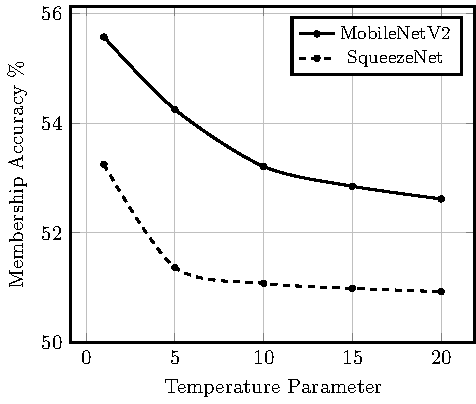
\includegraphics[width=0.7\columnwidth]{figures/efficientArch.pdf}
  \caption{The privacy leakage of off-the-shelf models is reduced by increasing the softmax temperature.}
  \label{softmax}
\end{figure}

Further, the membership inference accuracy of SqueezeNet and MobileNet can be further reduced close to random guess by increasing the temperature parameter of the softmax function applied to the output.
Increasing the temperature parameter reduces the granularity of the model's output and is given by $F_i(x) = e^{\frac{z_i(x)}{T}}$ / $ \sum_{j}e^{\frac{z_j(x)}{T}}$ where $z(x)$ computes output of the model before the softmax layer.
For the case of SqueezeNet, we are able to reduce the inference accuracy to 50.93\% from 53.07\% while for MobileNet we can reduce the inference accuracy to 52.62\% from 55.57\% as seen in Figure~\ref{softmax}.
This reduction in membership inference accuracy is without any cost of the prediction test accuracy of the model.




\subsubsection{Quantization}\label{quant}

In this section, we evaluate the technique of reducing the precision of both model's parameters and intermediate activations.
Further, we consider the extreme case of binarizing the parameters and activations allowing to evaluate on the most optimized case.
We evaluate on FashionMNIST dataset for two architectures with convolutional and fully connected layers as seen in Table~\ref{fmnist_quantize}.

\begin{table}[!htb]
\begin{center}
\renewcommand\arraystretch{1.5}
\fontsize{6.7pt}{6.7pt}\selectfont
\begin{tabular}{|c|c|c|c|c|}
\hline
\multicolumn{5}{|c|}{\textbf{FashionMNIST}}\\
\hline
\textbf{Architecture} & \textbf{Memory} & \textbf{Train}  & \textbf{Test}  & \textbf{Inference}  \\
 & \textbf{Accuracy} &  \textbf{Footprint} & \textbf{Accuracy} & \textbf{Accuracy}  \\
\hline
\multicolumn{5}{|c|}{Architecture 1}\\
Full & 38.39 MB & 100\% & 92.35\% & \cellcolor{red!25}57.46\%\\
BinaryNet & 1.62 MB & 88.68\% & 86.9\% & \cellcolor{green!25}55.45\%\\
XNOR-Net & 1.62 MB & 87.19\% & 85.68\% & \cellcolor{green!25}51.05\%\\ %1,626,824 parameters
\hline
\multicolumn{5}{|c|}{Architecture 2}\\
Full & 29.83 MB & 99.34\% & 89.88\% & \cellcolor{red!25}54.86\% \\
BinaryNet & 0.93 MB & 97.61\% & 89.60\% & \cellcolor{green!25}54.30\%\\
XNOR-Net & 0.93 MB & 92.67\% & 86.68\% & \cellcolor{green!25}51.74\%\\ %937,000parameters
\hline
\end{tabular}
\end{center}
\caption{Reducing the model precision lowers the inference attack accuracy but at the cost of test accuracy.}
\label{fmnist_quantize}
\end{table}

In both architectures, we see that computation on  binarized parameters and activations reduces the inference risk by a small value.
However, on replacing the MAC operations with XNOR operations, we observe that the inference risk decreases close to random guess, however, at the cost of prediction test accuracy.
The CIFAR10 results corresponding to the XNOR operations and its privacy comparison with full precision counterpart is indicated in Table~\ref{cifar10quant}.

In summary, we observe that quantization, specifically binarization of parameters and activation along with XNOR computation, provides strong resistance against inference attacks compared to model compression and off-the-shelf architectures.


%\begin{tcolorbox}[enhanced,attach boxed title to top center={yshift=-3mm,yshifttext=-1mm},
%  colback=gray!5!white,colframe=black!75!black,colbacktitle=gray!80!black,
%  title=Security Principle I,fonttitle=\bfseries,
%  boxed title style={size=small,colframe=black!50!black} ]
%Original inputs should not be revealed in the public cloud without proper protection.
%\end{tcolorbox}


\subsection{Summary of Comparison}
\label{eval-summary}

We summarize the properties satisfied by each of the technique in terms of privacy, computation, memory and energy efficiency in Table~\ref{tbl:comparison}.
Here, we mark the attributes which are satisfied with $\cmark$, requires additional hardware optimization as $\smark$ and does not satisfy the property with a $\xmark$.

\begin{table}[!htb]
\begin{center}
\renewcommand\arraystretch{1.5}
\fontsize{6.7pt}{6.7pt}\selectfont
\begin{tabular}{|l||l|l|l|}
\hline
Requirements & Compression & Quantization & Off-the-shelf  \\
\hline
Computation Efficiency & $\smark$  & $\cmark$   & $\xmark$ \\
\hline
Memory Efficiency &  $\smark$ & $\cmark$   & $\cmark$ \\
\hline
Energy Efficiency &  $\smark$   & $\cmark$   & $\xmark$ \\
\hline
Privacy &  $\xmark$   & $\cmark$   & $\smark$ \\
\hline
\end{tabular}
\end{center}
\caption{Only quantization satisfies all the requirements.}
%\caption{Comparison of different optimizations for NNs. $\smark$: additional hardware optimization; $\xmark$: requirement not satisfied; $\cmark$: requirement satisfied.}
\label{tbl:comparison}
\end{table}

In order to design NNs for embedded devices, quantization (binarization with XNOR computation) is an attractive design choice which not only satisfies the computation, memory and energy efficiency but also provides high resistance against inference attacks.
On the other hand, model compression without any weight sharing modifications, leaks more training data membership details making it significantly more vulnerable to membership inference attacks. Additionally, it requires hardware support and optimization to achieve better efficiency.
Off-the-shelf architectures, while provide decent privacy, does not satisfy all aspects of efficiency.
Hence, we choose quantization as a NN design for \method\hspace{0.01in} to provide a good three dimensional trade-off between privacy-efficiency-accuracy.


%\pgfplotsset{footnotesize,height=5.5cm,width=0.35\textwidth}
% \pgfplotsset{footnotesize,samples=10}

\begin{figure*}[ht!]
\begin{center}% note that \centering uses less vspace...
\resizebox{2\columnwidth}{!}{%
\begin{tabular}{lllll}


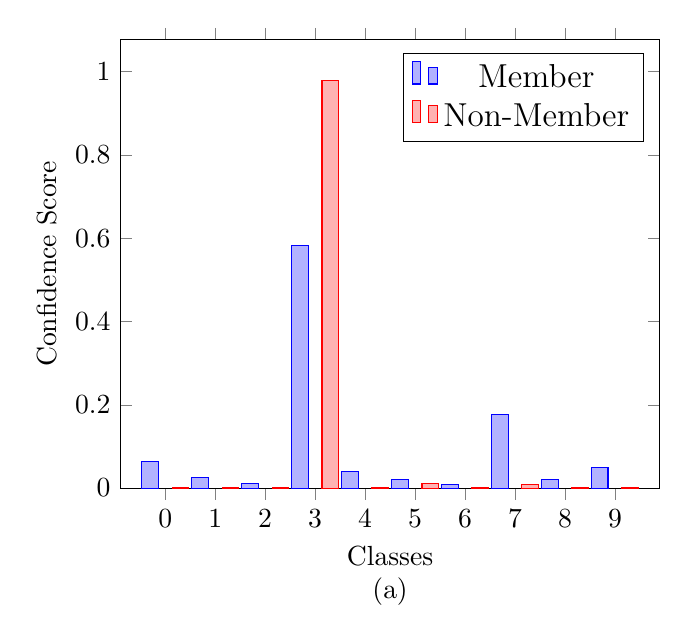
\begin{tikzpicture}
\begin{axis}[title={(a)},
title style={at={(0.5,0)},anchor=north,yshift=-35},
ylabel=Confidence Score,
xlabel=Classes,
legend style={font=\large},
legend pos =  north east,
ybar=5pt,% configures ‘bar shift’
bar width=6pt,
xtick={0,1,2,3,4,5,6,7,8,9},
ymin=0
]

\addplot
coordinates {(0,0.06327114254236221) (1,0.025417674332857132) (2,0.011714407242834568) (3,0.5831579566001892) (4,0.04046289622783661) (5,0.02152826450765133) (6,0.00799587182700634) (7,0.1768314242362976) (8,0.021124042570590973) (9,0.04849636182188988)};
\addplot
coordinates {(0,0.0010145490523427725) (1,0.00030558116850443184) (2,0.0008154626120813191) (3,0.9787409901618958) (4,0.00029880856163799763) (5,0.010064681060612202) (6,0.00022722511494066566) (7,0.007986118085682392) (8,0.00020130971097387373) (9,0.00034515938023105264)};

\legend{Member,Non-Member}
\end{axis}
\end{tikzpicture} &


%
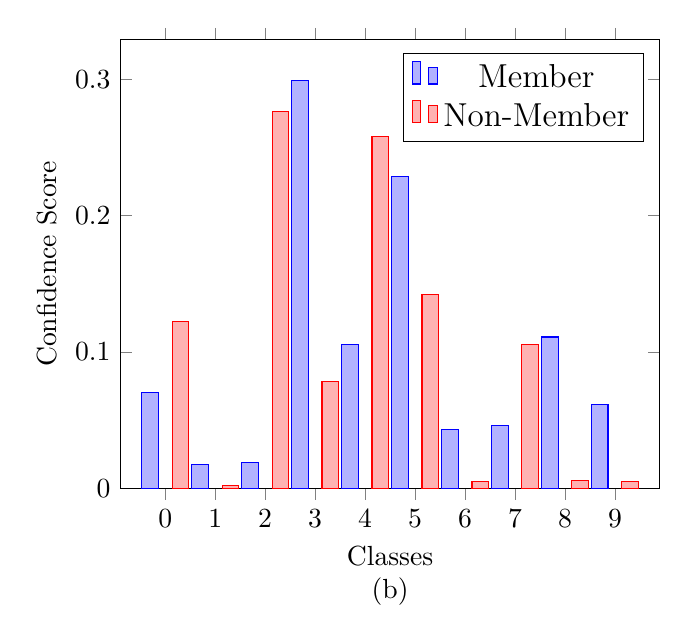
\begin{tikzpicture}
\begin{axis}[title={(b)},
title style={at={(0.5,0)},anchor=north,yshift=-35},
ylabel=Confidence Score,
xlabel=Classes,
xtick={0,1,2,3,4,5,6,7,8,9},
legend style={font=\large},
legend pos =  north east,
ybar=5pt,% configures ‘bar shift’
bar width=6pt,
ymin=0
]

\addplot
coordinates {(0,0.07000309228897095) (1,0.017400363460183144) (2,0.019030457362532616) (3,0.29907193779945374) (4,0.10515590757131577) (5,0.22833536565303802) (6,0.04266407713294029) (7,0.04584269970655441) (8,0.11086355894804001) (9,0.061632607132196426)};
\addplot
coordinates {(0,0.12253900617361069) (1,0.0015809950418770313) (2,0.27642616629600525) (3,0.07850959151983261) (4,0.2582301199436188) (5,0.14231687784194946) (6,0.004606064409017563) (7,0.10550655424594879) (8,0.005763859022408724) (9,0.004520699847489595)};

\legend{Member,Non-Member}
\end{axis}
\end{tikzpicture} &





%
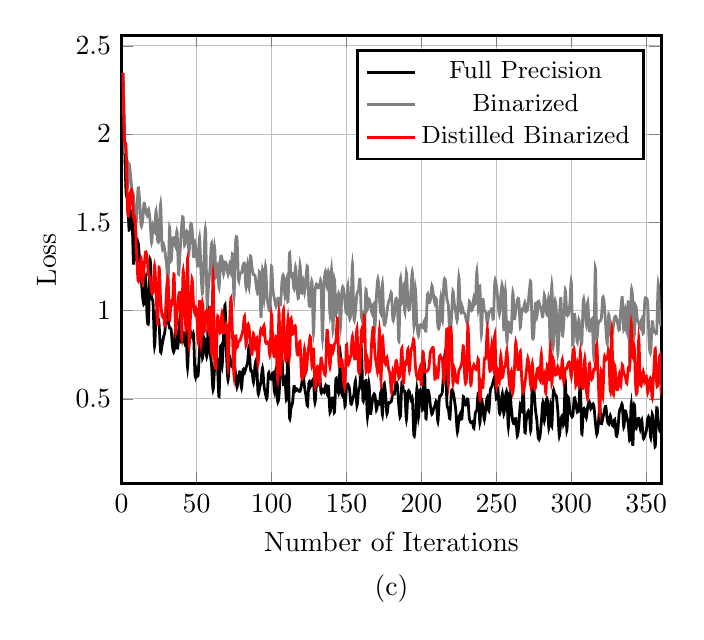
\begin{tikzpicture}
\begin{axis}[title={(c)},
title style={at={(0.5,0)},anchor=north,yshift=-35},
line width=1.0pt,
legend style={font=\small},
legend pos =  north east,
legend entries={Full Precision, Binarized, Distilled Binarized},
ylabel={Loss},
xmin=0,
xmax=360,
xlabel={Number of Iterations},
% extra x ticks={1,10,...,400},
% extra y ticks={0,0.5,...,10},
% extra y tick labels={},
% extra x tick labels={},
% extra x tick style={grid=major},
% extra y tick style={grid=major},
grid=major
]
\addplot[
    color=black,
    solid,
    smooth
    ]
    coordinates {
    ( 1 , 2.302968 )
    ( 2 , 1.939443 )
    ( 3 , 1.667299 )
    ( 4 , 1.652660 )
    ( 5 , 1.455838 )
    ( 6 , 1.559521 )
    ( 7 , 1.526025 )
    ( 8 , 1.260517 )
    ( 9 , 1.503018 )
    ( 10 , 1.285601 )
    ( 11 , 1.384281 )
    ( 12 , 1.286194 )
    ( 13 , 1.191418 )
    ( 14 , 1.079983 )
    ( 15 , 1.039906 )
    ( 16 , 1.188020 )
    ( 17 , 0.963824 )
    ( 18 , 0.943251 )
    ( 19 , 1.289535 )
    ( 20 , 1.082280 )
    ( 21 , 1.037991 )
    ( 22 , 0.799126 )
    ( 23 , 0.983668 )
    ( 24 , 0.966282 )
    ( 25 , 0.922792 )
    ( 26 , 0.765660 )
    ( 27 , 0.803365 )
    ( 28 , 0.850827 )
    ( 29 , 0.893062 )
    ( 30 , 1.063586 )
    ( 31 , 0.948933 )
    ( 32 , 0.901259 )
    ( 33 , 0.895251 )
    ( 34 , 0.794324 )
    ( 35 , 0.769924 )
    ( 36 , 0.899247 )
    ( 37 , 0.787751 )
    ( 38 , 0.831077 )
    ( 39 , 0.962390 )
    ( 40 , 0.821883 )
    ( 41 , 0.863004 )
    ( 42 , 0.818929 )
    ( 43 , 0.880331 )
    ( 44 , 0.676965 )
    ( 45 , 0.891206 )
    ( 46 , 0.876807 )
    ( 47 , 0.854072 )
    ( 48 , 0.860776 )
    ( 49 , 0.631650 )
    ( 50 , 0.662787 )
    ( 51 , 0.630878 )
    ( 52 , 0.778465 )
    ( 53 , 0.900262 )
    ( 54 , 0.731535 )
    ( 55 , 0.845547 )
    ( 56 , 0.785181 )
    ( 57 , 0.748590 )
    ( 58 , 0.986032 )
    ( 59 , 0.774422 )
    ( 60 , 0.691421 )
    ( 61 , 0.551147 )
    ( 62 , 0.668453 )
    ( 63 , 0.759031 )
    ( 64 , 0.673677 )
    ( 65 , 0.512989 )
    ( 66 , 0.796980 )
    ( 67 , 0.681779 )
    ( 68 , 0.851441 )
    ( 69 , 1.030697 )
    ( 70 , 0.751324 )
    ( 71 , 0.606460 )
    ( 72 , 0.733667 )
    ( 73 , 0.701998 )
    ( 74 , 0.680291 )
    ( 75 , 0.707206 )
    ( 76 , 0.645020 )
    ( 77 , 0.566519 )
    ( 78 , 0.622747 )
    ( 79 , 0.651569 )
    ( 80 , 0.560384 )
    ( 81 , 0.663585 )
    ( 82 , 0.648072 )
    ( 83 , 0.676273 )
    ( 84 , 0.701089 )
    ( 85 , 0.797614 )
    ( 86 , 0.665663 )
    ( 87 , 0.657626 )
    ( 88 , 0.592905 )
    ( 89 , 0.687644 )
    ( 90 , 0.712525 )
    ( 91 , 0.533854 )
    ( 92 , 0.557828 )
    ( 93 , 0.599991 )
    ( 94 , 0.673825 )
    ( 95 , 0.575448 )
    ( 96 , 0.526772 )
    ( 97 , 0.505667 )
    ( 98 , 0.643386 )
    ( 99 , 0.620009 )
    ( 100 , 0.610189 )
    ( 101 , 0.647692 )
    ( 102 , 0.539143 )
    ( 103 , 0.667260 )
    ( 104 , 0.489376 )
    ( 105 , 0.518314 )
    ( 106 , 0.676982 )
    ( 107 , 0.727331 )
    ( 108 , 0.581430 )
    ( 109 , 0.618056 )
    ( 110 , 0.500167 )
    ( 111 , 0.785589 )
    ( 112 , 0.399176 )
    ( 113 , 0.447618 )
    ( 114 , 0.475429 )
    ( 115 , 0.570146 )
    ( 116 , 0.544356 )
    ( 117 , 0.555152 )
    ( 118 , 0.546433 )
    ( 119 , 0.542349 )
    ( 120 , 0.577833 )
    ( 121 , 0.639318 )
    ( 122 , 0.567917 )
    ( 123 , 0.517693 )
    ( 124 , 0.460981 )
    ( 125 , 0.593507 )
    ( 126 , 0.570267 )
    ( 127 , 0.597812 )
    ( 128 , 0.598578 )
    ( 129 , 0.478810 )
    ( 130 , 0.586665 )
    ( 131 , 0.579736 )
    ( 132 , 0.659663 )
    ( 133 , 0.538597 )
    ( 134 , 0.549711 )
    ( 135 , 0.537823 )
    ( 136 , 0.572637 )
    ( 137 , 0.534132 )
    ( 138 , 0.570913 )
    ( 139 , 0.422553 )
    ( 140 , 0.488932 )
    ( 141 , 0.504971 )
    ( 142 , 0.423515 )
    ( 143 , 0.614434 )
    ( 144 , 0.564107 )
    ( 145 , 0.541557 )
    ( 146 , 0.744249 )
    ( 147 , 0.522557 )
    ( 148 , 0.606243 )
    ( 149 , 0.458936 )
    ( 150 , 0.558472 )
    ( 151 , 0.581740 )
    ( 152 , 0.556220 )
    ( 153 , 0.470633 )
    ( 154 , 0.493428 )
    ( 155 , 0.524618 )
    ( 156 , 0.601933 )
    ( 157 , 0.460702 )
    ( 158 , 0.542096 )
    ( 159 , 0.583347 )
    ( 160 , 0.778570 )
    ( 161 , 0.497549 )
    ( 162 , 0.533701 )
    ( 163 , 0.603471 )
    ( 164 , 0.397012 )
    ( 165 , 0.583966 )
    ( 166 , 0.417388 )
    ( 167 , 0.471393 )
    ( 168 , 0.520279 )
    ( 169 , 0.520528 )
    ( 170 , 0.437146 )
    ( 171 , 0.482065 )
    ( 172 , 0.469343 )
    ( 173 , 0.539111 )
    ( 174 , 0.408798 )
    ( 175 , 0.585470 )
    ( 176 , 0.532898 )
    ( 177 , 0.415162 )
    ( 178 , 0.476431 )
    ( 179 , 0.477853 )
    ( 180 , 0.486712 )
    ( 181 , 0.538571 )
    ( 182 , 0.526860 )
    ( 183 , 0.590460 )
    ( 184 , 0.575449 )
    ( 185 , 0.451290 )
    ( 186 , 0.401073 )
    ( 187 , 0.596629 )
    ( 188 , 0.545198 )
    ( 189 , 0.532833 )
    ( 190 , 0.382534 )
    ( 191 , 0.532536 )
    ( 192 , 0.539632 )
    ( 193 , 0.492966 )
    ( 194 , 0.496653 )
    ( 195 , 0.291686 )
    ( 196 , 0.359933 )
    ( 197 , 0.558284 )
    ( 198 , 0.393615 )
    ( 199 , 0.546782 )
    ( 200 , 0.507714 )
    ( 201 , 0.441790 )
    ( 202 , 0.694662 )
    ( 203 , 0.387495 )
    ( 204 , 0.539195 )
    ( 205 , 0.534799 )
    ( 206 , 0.460438 )
    ( 207 , 0.412882 )
    ( 208 , 0.439468 )
    ( 209 , 0.461498 )
    ( 210 , 0.484441 )
    ( 211 , 0.371391 )
    ( 212 , 0.505832 )
    ( 213 , 0.518648 )
    ( 214 , 0.544090 )
    ( 215 , 0.680713 )
    ( 216 , 0.751645 )
    ( 217 , 0.478645 )
    ( 218 , 0.442678 )
    ( 219 , 0.387577 )
    ( 220 , 0.538398 )
    ( 221 , 0.543274 )
    ( 222 , 0.495477 )
    ( 223 , 0.428225 )
    ( 224 , 0.311347 )
    ( 225 , 0.386528 )
    ( 226 , 0.415797 )
    ( 227 , 0.386841 )
    ( 228 , 0.512556 )
    ( 229 , 0.467811 )
    ( 230 , 0.469653 )
    ( 231 , 0.497145 )
    ( 232 , 0.386810 )
    ( 233 , 0.365984 )
    ( 234 , 0.370858 )
    ( 235 , 0.334157 )
    ( 236 , 0.421482 )
    ( 237 , 0.437231 )
    ( 238 , 0.533400 )
    ( 239 , 0.363779 )
    ( 240 , 0.499905 )
    ( 241 , 0.448234 )
    ( 242 , 0.381877 )
    ( 243 , 0.457827 )
    ( 244 , 0.508316 )
    ( 245 , 0.432367 )
    ( 246 , 0.550766 )
    ( 247 , 0.567483 )
    ( 248 , 0.600920 )
    ( 249 , 0.619330 )
    ( 250 , 0.501078 )
    ( 251 , 0.563693 )
    ( 252 , 0.420956 )
    ( 253 , 0.452368 )
    ( 254 , 0.529415 )
    ( 255 , 0.413688 )
    ( 256 , 0.507326 )
    ( 257 , 0.534332 )
    ( 258 , 0.340995 )
    ( 259 , 0.533992 )
    ( 260 , 0.445496 )
    ( 261 , 0.371866 )
    ( 262 , 0.357937 )
    ( 263 , 0.387621 )
    ( 264 , 0.290543 )
    ( 265 , 0.351936 )
    ( 266 , 0.467249 )
    ( 267 , 0.429069 )
    ( 268 , 0.564726 )
    ( 269 , 0.309757 )
    ( 270 , 0.382020 )
    ( 271 , 0.423434 )
    ( 272 , 0.425730 )
    ( 273 , 0.322237 )
    ( 274 , 0.597025 )
    ( 275 , 0.560745 )
    ( 276 , 0.445284 )
    ( 277 , 0.378794 )
    ( 278 , 0.276946 )
    ( 279 , 0.282341 )
    ( 280 , 0.366811 )
    ( 281 , 0.478299 )
    ( 282 , 0.375445 )
    ( 283 , 0.480307 )
    ( 284 , 0.493695 )
    ( 285 , 0.336665 )
    ( 286 , 0.462213 )
    ( 287 , 0.346743 )
    ( 288 , 0.541349 )
    ( 289 , 0.522342 )
    ( 290 , 0.514670 )
    ( 291 , 0.430172 )
    ( 292 , 0.289797 )
    ( 293 , 0.371195 )
    ( 294 , 0.405113 )
    ( 295 , 0.357373 )
    ( 296 , 0.603785 )
    ( 297 , 0.321793 )
    ( 298 , 0.506746 )
    ( 299 , 0.432704 )
    ( 300 , 0.405093 )
    ( 301 , 0.403066 )
    ( 302 , 0.504766 )
    ( 303 , 0.473787 )
    ( 304 , 0.425059 )
    ( 305 , 0.450767 )
    ( 306 , 0.582399 )
    ( 307 , 0.300974 )
    ( 308 , 0.433699 )
    ( 309 , 0.439344 )
    ( 310 , 0.394054 )
    ( 311 , 0.458976 )
    ( 312 , 0.482490 )
    ( 313 , 0.442764 )
    ( 314 , 0.467489 )
    ( 315 , 0.462829 )
    ( 316 , 0.372411 )
    ( 317 , 0.298418 )
    ( 318 , 0.353107 )
    ( 319 , 0.452360 )
    ( 320 , 0.359912 )
    ( 321 , 0.388992 )
    ( 322 , 0.428388 )
    ( 323 , 0.456512 )
    ( 324 , 0.380230 )
    ( 325 , 0.357444 )
    ( 326 , 0.403996 )
    ( 327 , 0.361251 )
    ( 328 , 0.344514 )
    ( 329 , 0.381908 )
    ( 330 , 0.289464 )
    ( 331 , 0.320182 )
    ( 332 , 0.425570 )
    ( 333 , 0.448104 )
    ( 334 , 0.466504 )
    ( 335 , 0.340016 )
    ( 336 , 0.430965 )
    ( 337 , 0.396781 )
    ( 338 , 0.356925 )
    ( 339 , 0.267577 )
    ( 340 , 0.468913 )
    ( 341 , 0.233512 )
    ( 342 , 0.466996 )
    ( 343 , 0.332996 )
    ( 344 , 0.367131 )
    ( 345 , 0.389329 )
    ( 346 , 0.330957 )
    ( 347 , 0.378960 )
    ( 348 , 0.278310 )
    ( 349 , 0.290548 )
    ( 350 , 0.316687 )
    ( 351 , 0.388542 )
    ( 352 , 0.388174 )
    ( 353 , 0.279368 )
    ( 354 , 0.412089 )
    ( 355 , 0.335098 )
    ( 356 , 0.229976 )
    ( 357 , 0.449180 )
    ( 358 , 0.374953 )
    ( 359 , 0.321231 )
    ( 360 , 0.348795 )
      };

      \addplot[
          color=gray,
          solid,
          smooth
          ]
          coordinates {
          ( 1 , 2.346761 )
  ( 2 , 1.926266 )
  ( 3 , 1.885543 )
  ( 4 , 1.695635 )
  ( 5 , 1.828619 )
  ( 6 , 1.763135 )
  ( 7 , 1.675170 )
  ( 8 , 1.648822 )
  ( 9 , 1.501599 )
  ( 10 , 1.517566 )
  ( 11 , 1.694481 )
  ( 12 , 1.630272 )
  ( 13 , 1.482632 )
  ( 14 , 1.509774 )
  ( 15 , 1.607969 )
  ( 16 , 1.573090 )
  ( 17 , 1.538904 )
  ( 18 , 1.573854 )
  ( 19 , 1.506782 )
  ( 20 , 1.384800 )
  ( 21 , 1.485137 )
  ( 22 , 1.445732 )
  ( 23 , 1.566089 )
  ( 24 , 1.400355 )
  ( 25 , 1.410617 )
  ( 26 , 1.602641 )
  ( 27 , 1.363793 )
  ( 28 , 1.374451 )
  ( 29 , 1.327962 )
  ( 30 , 1.259157 )
  ( 31 , 1.158507 )
  ( 32 , 1.471694 )
  ( 33 , 1.281064 )
  ( 34 , 1.395380 )
  ( 35 , 1.413245 )
  ( 36 , 1.364599 )
  ( 37 , 1.446778 )
  ( 38 , 1.205966 )
  ( 39 , 1.332203 )
  ( 40 , 1.474646 )
  ( 41 , 1.530147 )
  ( 42 , 1.370293 )
  ( 43 , 1.436183 )
  ( 44 , 1.444681 )
  ( 45 , 1.332167 )
  ( 46 , 1.484209 )
  ( 47 , 1.465831 )
  ( 48 , 1.305787 )
  ( 49 , 1.380785 )
  ( 50 , 1.305335 )
  ( 51 , 1.252715 )
  ( 52 , 1.414409 )
  ( 53 , 1.208195 )
  ( 54 , 1.097216 )
  ( 55 , 1.304714 )
  ( 56 , 1.456459 )
  ( 57 , 1.040485 )
  ( 58 , 1.141915 )
  ( 59 , 1.240699 )
  ( 60 , 1.379954 )
  ( 61 , 1.174325 )
  ( 62 , 1.360094 )
  ( 63 , 1.193203 )
  ( 64 , 1.246328 )
  ( 65 , 1.128607 )
  ( 66 , 1.297393 )
  ( 67 , 1.293353 )
  ( 68 , 1.207303 )
  ( 69 , 1.274779 )
  ( 70 , 1.260201 )
  ( 71 , 1.205472 )
  ( 72 , 1.257582 )
  ( 73 , 1.209281 )
  ( 74 , 1.320339 )
  ( 75 , 1.081225 )
  ( 76 , 1.379258 )
  ( 77 , 1.403371 )
  ( 78 , 1.173059 )
  ( 79 , 1.210906 )
  ( 80 , 1.212522 )
  ( 81 , 1.256900 )
  ( 82 , 1.261412 )
  ( 83 , 1.132829 )
  ( 84 , 1.261608 )
  ( 85 , 1.130152 )
  ( 86 , 1.307679 )
  ( 87 , 1.242157 )
  ( 88 , 1.203381 )
  ( 89 , 1.197875 )
  ( 90 , 1.127777 )
  ( 91 , 1.099596 )
  ( 92 , 1.218491 )
  ( 93 , 0.959279 )
  ( 94 , 1.230520 )
  ( 95 , 1.063139 )
  ( 96 , 1.248715 )
  ( 97 , 1.083069 )
  ( 98 , 1.019647 )
  ( 99 , 1.012220 )
  ( 100 , 1.250834 )
  ( 101 , 1.113485 )
  ( 102 , 1.065619 )
  ( 103 , 1.023666 )
  ( 104 , 1.063910 )
  ( 105 , 1.067258 )
  ( 106 , 1.032276 )
  ( 107 , 1.165910 )
  ( 108 , 1.197135 )
  ( 109 , 1.079468 )
  ( 110 , 1.176466 )
  ( 111 , 1.049984 )
  ( 112 , 1.325067 )
  ( 113 , 1.198396 )
  ( 114 , 1.209702 )
  ( 115 , 1.122866 )
  ( 116 , 1.246204 )
  ( 117 , 1.130638 )
  ( 118 , 1.070367 )
  ( 119 , 1.258520 )
  ( 120 , 1.100373 )
  ( 121 , 1.169035 )
  ( 122 , 1.103153 )
  ( 123 , 1.187527 )
  ( 124 , 1.249404 )
  ( 125 , 1.039255 )
  ( 126 , 1.043600 )
  ( 127 , 1.163061 )
  ( 128 , 0.866229 )
  ( 129 , 1.100545 )
  ( 130 , 1.150101 )
  ( 131 , 1.129426 )
  ( 132 , 1.129657 )
  ( 133 , 1.159651 )
  ( 134 , 0.838983 )
  ( 135 , 1.136622 )
  ( 136 , 1.221408 )
  ( 137 , 1.139824 )
  ( 138 , 1.213746 )
  ( 139 , 0.979337 )
  ( 140 , 1.232616 )
  ( 141 , 0.885131 )
  ( 142 , 1.174824 )
  ( 143 , 0.979129 )
  ( 144 , 1.055910 )
  ( 145 , 1.090147 )
  ( 146 , 0.904567 )
  ( 147 , 1.113498 )
  ( 148 , 1.125462 )
  ( 149 , 1.049405 )
  ( 150 , 0.985949 )
  ( 151 , 1.139380 )
  ( 152 , 0.959967 )
  ( 153 , 1.000041 )
  ( 154 , 1.263282 )
  ( 155 , 0.956478 )
  ( 156 , 0.995327 )
  ( 157 , 1.096886 )
  ( 158 , 1.111590 )
  ( 159 , 1.176757 )
  ( 160 , 0.962864 )
  ( 161 , 0.977689 )
  ( 162 , 0.922844 )
  ( 163 , 1.120963 )
  ( 164 , 1.009984 )
  ( 165 , 1.063984 )
  ( 166 , 1.032832 )
  ( 167 , 0.987173 )
  ( 168 , 1.035523 )
  ( 169 , 0.903309 )
  ( 170 , 1.083587 )
  ( 171 , 1.178625 )
  ( 172 , 1.068447 )
  ( 173 , 0.984077 )
  ( 174 , 1.152232 )
  ( 175 , 0.932497 )
  ( 176 , 0.932060 )
  ( 177 , 0.994724 )
  ( 178 , 1.047627 )
  ( 179 , 1.068406 )
  ( 180 , 1.097718 )
  ( 181 , 0.946308 )
  ( 182 , 0.981098 )
  ( 183 , 1.067997 )
  ( 184 , 1.027874 )
  ( 185 , 0.826300 )
  ( 186 , 1.179658 )
  ( 187 , 1.052969 )
  ( 188 , 1.142715 )
  ( 189 , 0.991129 )
  ( 190 , 1.213003 )
  ( 191 , 1.045486 )
  ( 192 , 1.006147 )
  ( 193 , 1.109902 )
  ( 194 , 1.212793 )
  ( 195 , 0.912005 )
  ( 196 , 1.123085 )
  ( 197 , 0.926187 )
  ( 198 , 0.858419 )
  ( 199 , 0.916872 )
  ( 200 , 0.915458 )
  ( 201 , 0.904451 )
  ( 202 , 0.942618 )
  ( 203 , 0.883013 )
  ( 204 , 1.090961 )
  ( 205 , 1.045205 )
  ( 206 , 1.059832 )
  ( 207 , 1.141301 )
  ( 208 , 1.089335 )
  ( 209 , 1.039749 )
  ( 210 , 1.063170 )
  ( 211 , 0.912232 )
  ( 212 , 0.915569 )
  ( 213 , 1.075158 )
  ( 214 , 0.940946 )
  ( 215 , 1.157747 )
  ( 216 , 1.170259 )
  ( 217 , 1.066205 )
  ( 218 , 1.024397 )
  ( 219 , 0.852790 )
  ( 220 , 0.950637 )
  ( 221 , 1.110507 )
  ( 222 , 1.036702 )
  ( 223 , 0.984222 )
  ( 224 , 0.952827 )
  ( 225 , 1.188724 )
  ( 226 , 1.000404 )
  ( 227 , 1.028348 )
  ( 228 , 0.988035 )
  ( 229 , 0.983033 )
  ( 230 , 0.942389 )
  ( 231 , 0.935704 )
  ( 232 , 1.051824 )
  ( 233 , 1.005647 )
  ( 234 , 1.006882 )
  ( 235 , 1.072922 )
  ( 236 , 1.043638 )
  ( 237 , 1.221575 )
  ( 238 , 1.003483 )
  ( 239 , 1.138196 )
  ( 240 , 0.862098 )
  ( 241 , 1.062384 )
  ( 242 , 0.999307 )
  ( 243 , 0.991120 )
  ( 244 , 0.926649 )
  ( 245 , 0.986342 )
  ( 246 , 0.992192 )
  ( 247 , 1.010563 )
  ( 248 , 0.952089 )
  ( 249 , 1.165234 )
  ( 250 , 1.141195 )
  ( 251 , 1.059924 )
  ( 252 , 0.980622 )
  ( 253 , 1.091556 )
  ( 254 , 1.136913 )
  ( 255 , 0.883962 )
  ( 256 , 1.111804 )
  ( 257 , 0.826448 )
  ( 258 , 0.934091 )
  ( 259 , 0.895227 )
  ( 260 , 0.889213 )
  ( 261 , 1.103202 )
  ( 262 , 0.953661 )
  ( 263 , 1.005441 )
  ( 264 , 1.058801 )
  ( 265 , 1.057636 )
  ( 266 , 0.903979 )
  ( 267 , 1.003013 )
  ( 268 , 1.001371 )
  ( 269 , 1.045060 )
  ( 270 , 0.995644 )
  ( 271 , 1.017072 )
  ( 272 , 1.109493 )
  ( 273 , 1.156392 )
  ( 274 , 0.859848 )
  ( 275 , 0.867010 )
  ( 276 , 1.039820 )
  ( 277 , 0.963619 )
  ( 278 , 1.051263 )
  ( 279 , 1.029461 )
  ( 280 , 1.002586 )
  ( 281 , 0.965037 )
  ( 282 , 1.089420 )
  ( 283 , 1.019706 )
  ( 284 , 0.973446 )
  ( 285 , 1.068585 )
  ( 286 , 0.790222 )
  ( 287 , 1.146344 )
  ( 288 , 0.802443 )
  ( 289 , 1.046202 )
  ( 290 , 0.997245 )
  ( 291 , 0.754709 )
  ( 292 , 0.945580 )
  ( 293 , 1.069640 )
  ( 294 , 0.858742 )
  ( 295 , 0.934347 )
  ( 296 , 1.114184 )
  ( 297 , 0.985928 )
  ( 298 , 0.977279 )
  ( 299 , 1.034217 )
  ( 300 , 1.159927 )
  ( 301 , 0.804602 )
  ( 302 , 0.978465 )
  ( 303 , 0.916436 )
  ( 304 , 0.819233 )
  ( 305 , 0.947365 )
  ( 306 , 0.873999 )
  ( 307 , 0.814669 )
  ( 308 , 1.060480 )
  ( 309 , 1.009367 )
  ( 310 , 0.923004 )
  ( 311 , 1.046344 )
  ( 312 , 0.884677 )
  ( 313 , 0.931433 )
  ( 314 , 0.941696 )
  ( 315 , 0.756139 )
  ( 316 , 1.241746 )
  ( 317 , 0.852658 )
  ( 318 , 0.924763 )
  ( 319 , 0.942495 )
  ( 320 , 0.954869 )
  ( 321 , 1.075119 )
  ( 322 , 1.036582 )
  ( 323 , 0.906247 )
  ( 324 , 0.812499 )
  ( 325 , 0.977565 )
  ( 326 , 0.870054 )
  ( 327 , 0.857418 )
  ( 328 , 0.904272 )
  ( 329 , 0.964146 )
  ( 330 , 0.960810 )
  ( 331 , 0.922262 )
  ( 332 , 0.889789 )
  ( 333 , 1.004996 )
  ( 334 , 1.073944 )
  ( 335 , 0.891395 )
  ( 336 , 1.000604 )
  ( 337 , 0.882347 )
  ( 338 , 1.048631 )
  ( 339 , 0.699180 )
  ( 340 , 1.102788 )
  ( 341 , 1.062422 )
  ( 342 , 0.861747 )
  ( 343 , 1.025133 )
  ( 344 , 0.951212 )
  ( 345 , 0.927888 )
  ( 346 , 0.904762 )
  ( 347 , 0.950766 )
  ( 348 , 0.868892 )
  ( 349 , 1.051545 )
  ( 350 , 1.070194 )
  ( 351 , 1.035250 )
  ( 352 , 0.803139 )
  ( 353 , 0.765967 )
  ( 354 , 0.936454 )
  ( 355 , 0.882868 )
  ( 356 , 0.877807 )
  ( 357 , 0.886292 )
  ( 358 , 1.150183 )
  ( 359 , 0.951342 )
  ( 360 , 0.913005 )
            };

  \addplot[
      color=red,
      solid,
      smooth
      ]
      coordinates {
      ( 1 , 2.346761 )
      ( 1 , 2.289508 )
      ( 2 , 1.958497 )
      ( 3 , 1.921034 )
      ( 4 , 1.561351 )
      ( 5 , 1.560222 )
      ( 6 , 1.672546 )
      ( 7 , 1.671921 )
      ( 8 , 1.527745 )
      ( 9 , 1.516091 )
      ( 10 , 1.320806 )
      ( 11 , 1.168530 )
      ( 12 , 1.210074 )
      ( 13 , 1.297815 )
      ( 14 , 1.161482 )
      ( 15 , 1.246961 )
      ( 16 , 1.331731 )
      ( 17 , 1.299713 )
      ( 18 , 1.200435 )
      ( 19 , 1.183215 )
      ( 20 , 1.105063 )
      ( 21 , 1.109861 )
      ( 22 , 1.254844 )
      ( 23 , 1.108233 )
      ( 24 , 0.924076 )
      ( 25 , 1.244691 )
      ( 26 , 1.063551 )
      ( 27 , 0.970651 )
      ( 28 , 0.976295 )
      ( 29 , 0.913169 )
      ( 30 , 1.119265 )
      ( 31 , 1.173765 )
      ( 32 , 0.947561 )
      ( 33 , 1.054491 )
      ( 34 , 1.046588 )
      ( 35 , 1.206818 )
      ( 36 , 0.882458 )
      ( 37 , 0.983017 )
      ( 38 , 1.080579 )
      ( 39 , 1.086890 )
      ( 40 , 0.842886 )
      ( 41 , 1.221012 )
      ( 42 , 1.075716 )
      ( 43 , 0.899074 )
      ( 44 , 1.293818 )
      ( 45 , 0.811225 )
      ( 46 , 0.981191 )
      ( 47 , 1.177047 )
      ( 48 , 1.032480 )
      ( 49 , 0.981890 )
      ( 50 , 1.005604 )
      ( 51 , 0.828696 )
      ( 52 , 1.057695 )
      ( 53 , 0.824240 )
      ( 54 , 1.040227 )
      ( 55 , 0.879299 )
      ( 56 , 0.971962 )
      ( 57 , 0.997197 )
      ( 58 , 0.886545 )
      ( 59 , 1.017593 )
      ( 60 , 0.762022 )
      ( 61 , 1.199266 )
      ( 62 , 0.736034 )
      ( 63 , 0.687340 )
      ( 64 , 0.962291 )
      ( 65 , 0.905756 )
      ( 66 , 0.875405 )
      ( 67 , 0.986668 )
      ( 68 , 0.885548 )
      ( 69 , 0.877220 )
      ( 70 , 0.914856 )
      ( 71 , 0.682138 )
      ( 72 , 0.919164 )
      ( 73 , 1.070877 )
      ( 74 , 0.855854 )
      ( 75 , 0.627857 )
      ( 76 , 0.856239 )
      ( 77 , 0.792077 )
      ( 78 , 0.823261 )
      ( 79 , 0.830847 )
      ( 80 , 0.857799 )
      ( 81 , 0.892394 )
      ( 82 , 0.966335 )
      ( 83 , 0.803680 )
      ( 84 , 0.914873 )
      ( 85 , 0.908078 )
      ( 86 , 0.798237 )
      ( 87 , 0.752717 )
      ( 88 , 0.869953 )
      ( 89 , 0.796312 )
      ( 90 , 0.844140 )
      ( 91 , 0.699578 )
      ( 92 , 0.830843 )
      ( 93 , 0.896852 )
      ( 94 , 0.871961 )
      ( 95 , 0.915021 )
      ( 96 , 0.821148 )
      ( 97 , 0.817516 )
      ( 98 , 0.820520 )
      ( 99 , 0.750622 )
      ( 100 , 0.976288 )
      ( 101 , 0.791571 )
      ( 102 , 0.738218 )
      ( 103 , 0.854439 )
      ( 104 , 0.610627 )
      ( 105 , 0.990846 )
      ( 106 , 0.649290 )
      ( 107 , 0.813209 )
      ( 108 , 1.002776 )
      ( 109 , 0.739490 )
      ( 110 , 0.742654 )
      ( 111 , 0.952149 )
      ( 112 , 0.742725 )
      ( 113 , 0.953895 )
      ( 114 , 0.866470 )
      ( 115 , 0.899595 )
      ( 116 , 0.905452 )
      ( 117 , 0.761735 )
      ( 118 , 0.759309 )
      ( 119 , 0.824847 )
      ( 120 , 0.632895 )
      ( 121 , 0.629622 )
      ( 122 , 0.782615 )
      ( 123 , 0.652874 )
      ( 124 , 0.728099 )
      ( 125 , 0.806889 )
      ( 126 , 0.848280 )
      ( 127 , 0.685887 )
      ( 128 , 0.781918 )
      ( 129 , 0.568329 )
      ( 130 , 0.653542 )
      ( 131 , 0.681325 )
      ( 132 , 0.587069 )
      ( 133 , 0.728819 )
      ( 134 , 0.688508 )
      ( 135 , 0.655295 )
      ( 136 , 0.647998 )
      ( 137 , 0.887438 )
      ( 138 , 0.804118 )
      ( 139 , 0.681075 )
      ( 140 , 0.801215 )
      ( 141 , 0.765510 )
      ( 142 , 0.810749 )
      ( 143 , 0.832472 )
      ( 144 , 0.954358 )
      ( 145 , 0.698934 )
      ( 146 , 0.696781 )
      ( 147 , 0.720781 )
      ( 148 , 0.611648 )
      ( 149 , 0.570984 )
      ( 150 , 0.805634 )
      ( 151 , 0.698532 )
      ( 152 , 0.715090 )
      ( 153 , 0.752225 )
      ( 154 , 0.854783 )
      ( 155 , 0.743349 )
      ( 156 , 0.737030 )
      ( 157 , 0.898713 )
      ( 158 , 0.668182 )
      ( 159 , 0.672265 )
      ( 160 , 0.889392 )
      ( 161 , 0.825691 )
      ( 162 , 0.970438 )
      ( 163 , 0.662543 )
      ( 164 , 0.723655 )
      ( 165 , 0.652735 )
      ( 166 , 0.684006 )
      ( 167 , 0.844469 )
      ( 168 , 0.903263 )
      ( 169 , 0.756717 )
      ( 170 , 0.695948 )
      ( 171 , 0.658278 )
      ( 172 , 0.890274 )
      ( 173 , 0.604330 )
      ( 174 , 0.846531 )
      ( 175 , 0.740486 )
      ( 176 , 0.697799 )
      ( 177 , 0.732877 )
      ( 178 , 0.674738 )
      ( 179 , 0.642503 )
      ( 180 , 0.539443 )
      ( 181 , 0.657330 )
      ( 182 , 0.605968 )
      ( 183 , 0.715463 )
      ( 184 , 0.682130 )
      ( 185 , 0.617121 )
      ( 186 , 0.661775 )
      ( 187 , 0.788635 )
      ( 188 , 0.588687 )
      ( 189 , 0.700439 )
      ( 190 , 0.697120 )
      ( 191 , 0.781461 )
      ( 192 , 0.660160 )
      ( 193 , 0.770010 )
      ( 194 , 0.800414 )
      ( 195 , 0.835379 )
      ( 196 , 0.684457 )
      ( 197 , 0.623300 )
      ( 198 , 0.611837 )
      ( 199 , 0.672864 )
      ( 200 , 0.579889 )
      ( 201 , 0.766305 )
      ( 202 , 0.661602 )
      ( 203 , 0.654130 )
      ( 204 , 0.659236 )
      ( 205 , 0.676831 )
      ( 206 , 0.763144 )
      ( 207 , 0.783112 )
      ( 208 , 0.779393 )
      ( 209 , 0.611283 )
      ( 210 , 0.660481 )
      ( 211 , 0.622174 )
      ( 212 , 0.739116 )
      ( 213 , 0.736537 )
      ( 214 , 0.717488 )
      ( 215 , 0.603474 )
      ( 216 , 0.720956 )
      ( 217 , 0.895162 )
      ( 218 , 0.583987 )
      ( 219 , 0.885873 )
      ( 220 , 0.865381 )
      ( 221 , 0.591229 )
      ( 222 , 0.669389 )
      ( 223 , 0.612504 )
      ( 224 , 0.592590 )
      ( 225 , 0.660891 )
      ( 226 , 0.677134 )
      ( 227 , 0.708002 )
      ( 228 , 0.798415 )
      ( 229 , 0.613641 )
      ( 230 , 0.610063 )
      ( 231 , 0.912058 )
      ( 232 , 0.711359 )
      ( 233 , 0.578273 )
      ( 234 , 0.661869 )
      ( 235 , 0.692462 )
      ( 236 , 0.670032 )
      ( 237 , 0.670372 )
      ( 238 , 0.722965 )
      ( 239 , 0.490983 )
      ( 240 , 0.599413 )
      ( 241 , 0.564405 )
      ( 242 , 0.720429 )
      ( 243 , 0.738146 )
      ( 244 , 0.895175 )
      ( 245 , 0.716247 )
      ( 246 , 0.657736 )
      ( 247 , 0.809308 )
      ( 248 , 0.673177 )
      ( 249 , 0.861484 )
      ( 250 , 0.572226 )
      ( 251 , 0.659255 )
      ( 252 , 0.596616 )
      ( 253 , 0.746455 )
      ( 254 , 0.621354 )
      ( 255 , 0.668629 )
      ( 256 , 0.692351 )
      ( 257 , 0.772648 )
      ( 258 , 0.658080 )
      ( 259 , 0.568799 )
      ( 260 , 0.655683 )
      ( 261 , 0.536369 )
      ( 262 , 0.655911 )
      ( 263 , 0.821214 )
      ( 264 , 0.690711 )
      ( 265 , 0.666788 )
      ( 266 , 0.769021 )
      ( 267 , 0.603920 )
      ( 268 , 0.538827 )
      ( 269 , 0.586855 )
      ( 270 , 0.653802 )
      ( 271 , 0.729698 )
      ( 272 , 0.662506 )
      ( 273 , 0.573307 )
      ( 274 , 0.698765 )
      ( 275 , 0.571538 )
      ( 276 , 0.560311 )
      ( 277 , 0.653228 )
      ( 278 , 0.674414 )
      ( 279 , 0.609833 )
      ( 280 , 0.754565 )
      ( 281 , 0.590132 )
      ( 282 , 0.637046 )
      ( 283 , 0.533268 )
      ( 284 , 0.690426 )
      ( 285 , 0.608395 )
      ( 286 , 0.782570 )
      ( 287 , 0.586600 )
      ( 288 , 0.720135 )
      ( 289 , 0.644524 )
      ( 290 , 0.636831 )
      ( 291 , 0.682296 )
      ( 292 , 0.644609 )
      ( 293 , 0.619640 )
      ( 294 , 0.721622 )
      ( 295 , 0.595761 )
      ( 296 , 0.669771 )
      ( 297 , 0.672078 )
      ( 298 , 0.702717 )
      ( 299 , 0.700702 )
      ( 300 , 0.623715 )
      ( 301 , 0.752632 )
      ( 302 , 0.772183 )
      ( 303 , 0.574867 )
      ( 304 , 0.694724 )
      ( 305 , 0.579246 )
      ( 306 , 0.763784 )
      ( 307 , 0.584890 )
      ( 308 , 0.568738 )
      ( 309 , 0.728641 )
      ( 310 , 0.555155 )
      ( 311 , 0.508444 )
      ( 312 , 0.696937 )
      ( 313 , 0.616997 )
      ( 314 , 0.615176 )
      ( 315 , 0.667652 )
      ( 316 , 0.675299 )
      ( 317 , 0.810867 )
      ( 318 , 0.603052 )
      ( 319 , 0.418517 )
      ( 320 , 0.652455 )
      ( 321 , 0.513917 )
      ( 322 , 0.730091 )
      ( 323 , 0.720278 )
      ( 324 , 0.729959 )
      ( 325 , 0.768966 )
      ( 326 , 0.547639 )
      ( 327 , 0.893457 )
      ( 328 , 0.526425 )
      ( 329 , 0.687370 )
      ( 330 , 0.572277 )
      ( 331 , 0.553026 )
      ( 332 , 0.636406 )
      ( 333 , 0.578816 )
      ( 334 , 0.692453 )
      ( 335 , 0.641644 )
      ( 336 , 0.629935 )
      ( 337 , 0.588312 )
      ( 338 , 0.677901 )
      ( 339 , 0.682241 )
      ( 340 , 0.924726 )
      ( 341 , 0.736128 )
      ( 342 , 0.794371 )
      ( 343 , 0.559741 )
      ( 344 , 0.550659 )
      ( 345 , 0.842112 )
      ( 346 , 0.594323 )
      ( 347 , 0.587956 )
      ( 348 , 0.653175 )
      ( 349 , 0.598934 )
      ( 350 , 0.627735 )
      ( 351 , 0.535564 )
      ( 352 , 0.593137 )
      ( 353 , 0.614303 )
      ( 354 , 0.503203 )
      ( 355 , 0.654863 )
      ( 356 , 0.783821 )
      ( 357 , 0.581702 )
      ( 358 , 0.599832 )
      ( 359 , 0.742905 )
      ( 360 , 0.518803 )
        };

\end{axis}
\end{tikzpicture}
\end{tabular}
}
\caption{(a) The confidence scores are distinguishable between train and test data records in undefended models trained making them vulnerable to membership inference attacks. (b) \method\hspace{0.02in} models have indistinguishable confidence scores. (c) The loss trajectories in Phase I is higher than Phase II indicating the improvement in accuracy.}
\label{fig:loss}
\end{center}
\end{figure*}


\subsection{Evaluating Phase I}
\label{evalPh1}

In Phase I of \method, we quantize the model and replace the MACs with cheap XNOR operations.
We observe that the inference attack accuracy decreases significantly for all the three architecture close to random guess ($\sim$50\%).
Specifically, the inference accuracy decreases from 56.69\% to 51.76\% for NiN, 60.40\% to 51.40\% for AlexNet and 58.70\% to 52.65\% for VGGNet.


\begin{table}[!htb]
\begin{center}
\renewcommand\arraystretch{1.5}
\fontsize{6.7pt}{6.7pt}\selectfont
\begin{tabular}{|c|c|c|c|c|}
\hline
\multicolumn{5}{|c|}{\textbf{CIFAR10}} \\
\hline
\multicolumn{2}{|c|}{\textbf{Architecture}} & \textbf{Train}  & \textbf{Test}  & \textbf{Inference}  \\
 \multicolumn{2}{|c|}{} & \textbf{Accuracy} & \textbf{Accuracy} & \textbf{Accuracy}  \\
\hline
\multirow{2}{*}{NiN} & Full Precision & 98.16\% & 86.16\% & \cellcolor{red!25}56.69\% \\
& Binary Precision & 81.93\% & 78.74\% & \cellcolor{green!25}51.76\% \\
\hline
\multirow{2}{*}{AlexNet} & Full Precision & 97.86\% & 80.34\% & \cellcolor{red!25}60.40\% \\
& Binary Precision & 68.62\% & 66.8\% & \cellcolor{green!25}51.40\% \\
\hline
\multirow{2}{*}{VGG13} & Full Precision & 99.58\% & 88.95\% & \cellcolor{red!25}58.70\%\\
& Binary Precision & 79.67\% & 74.64\% & \cellcolor{green!25}52.65\%\\
\hline
\end{tabular}
\end{center}
\caption{Reducing the precision of models lowers the membership privacy leakage but at the cost of accuracy.}
%through membership inference attacks
\label{cifar10quant}
\end{table}


However, since Phase I only optimizes the network for privacy and efficiency, the resultant model shows poor utility (accuracy).
We observe a significant loss in test accuracy for all the three models: around 8\% accuracy drop from 86.16\% to 78.74\% for NiN; 14\% accuracy drop from 80.34\% to 66.8\% for AlexNet; 14\% for VGG model from 88.95\% to 74.64\%.
In order to restore the accuracy, we use knowledge distillation as described in Phase II of the \method\hspace{0.02in} framework.

The privacy provided by quantized NN is due to the decrease in overfitting, empirically measured using the difference between the train and test accuracy.
The leakage in inference accuracy is attributed to the higher overfitting in models as well as memorization of the training data information in the form of the parameters, which are specifically tuned to achieve high performance on the train data~\cite{10.1145/3133956.3134077,236216,DBLP:journals/corr/abs-1812-00910}.
This is attributed to the reduction in learning capacity of the model on quantizing the parameters which lowers the sensitive training data information memorized by the parameters on lowering the precision.
Further, the quantization acts as a noise to strongly regularize the model~\cite{NIPS2016_6573}.
At the same time, this optimization provides high degree of efficiency to be executed on low powered embedded devices.

\subsection{Evaluating Phase II}
\label{evalPh2}

The objective of Phase II of \method\hspace{0.02in} is to enhance the accuracy of the quantized model with XNOR computations which depicts high inference attack resistance and efficiency.
In Phase II, we use the teacher-student model (described in Section~\ref{design}) to train the quantized student model being guided using the output predictions of the full precision teacher model.
Here, Phase II is heterogeneous, i.e, we are flexible to choose any full precision teacher model which can provide high accuracy on the considered dataset (Table~\ref{kd}).
Here, we consider pre-trained state of the art architectures\footnote{https://github.com/huyvnphan/PyTorch\_CIFAR10}: DenseNet169 and ResNet50, along with the full precision versions of NiN, Alexnet and VGGNet.
The standalone test accuracy of the DenseNet169 and ResNet50 architectures are 92.84\% and 92.12\% respectively with inference accuracy around to 55\% while the full precision accuracies for NiN, AlexNet and VGGNet are given in Table~\ref{cifar10quant}.


\begin{table}[!htb]
\begin{center}
\renewcommand\arraystretch{1.5}
\fontsize{6.7pt}{6.7pt}\selectfont
\begin{tabular}{|c|c|c|c|c|c|}
\hline
\textbf{Teacher} & \textbf{Student} & \textbf{Train}  & \textbf{Test}  & \textbf{Inference}  \\
&  & \textbf{Accuracy} & \textbf{Accuracy} & \textbf{Accuracy}  \\
\hline
\multicolumn{5}{|c|}{Standalone Models}\\
\hline
Binary NiN & None & 81.93\% & 78.74\% & 51.76\% \\
Binary AlexNet & None & 68.62\% & 66.8\% & 51.40\% \\
Binary VGG13 & None & 79.67\% & 74.64\% & 52.65\%\\
\hline
\multicolumn{5}{|c|}{Homogeneous Architecture Distillation}\\
\hline
NiN & Binary NiN & 90.49\% & 83.52\% & 53.90\% \\
AlexNet & Binary AlexNet & 76.79\% & 73.5\% & 51.85\% \\
VGG13 & Binary VGG13 & 89.45\% & 81.58\% & 54.98\%\\
\hline
\multicolumn{5}{|c|}{Heterogeneous Architecture Distillation}\\
\hline
DenseNet169 & NiN & 92.84\% & 83.71\% & 54.95\%\\
DenseNet169 & AlexNet & 81.87\% & 76.23\% & 53.51\%\\
DenseNet169 & VGG13 & 93.45\% & 85.8\% & 54.17\%\\
\hline
ResNet50 & NiN & 91.74\% & 83.77\% & 54.53\% \\
ResNet50 & AlexNet & 80.12\% & 74.92\% & 53.12\%\\
ResNet50 & VGG13 & 94.23\% & 86.52\% & 54.46\%\\
\hline
\end{tabular}
\end{center}
\caption{Phase II of \method\hspace{0.02in} improves the accuracy of the private-efficient model from Phase I.}
\label{kd}
\vspace{-0.3in}
\end{table}


The first set of experiments combine the same full precision model architectures with the quantized model versions, i.e, full precision NiN with Binarized NiN (homogeneous knowledge distillation).
Here, we see that there is 5\% increase in test accuracy (from 78.74\% to 83.52\%) for NiN with an increase of 2\% in inference attack.
Similarly, there is an increase of 7\% test accuracy for AlexNet with a very minimal privacy leakage increase of 0.45\%; and increase of 7\% test accuracy at the cost of 2\% inference attack accuracy for VGGNet.
For heterogeneous knowledge distillation, i.e, combining other architectures (DenseNet169 and ResNet50) with the quantized models from Phase I, we see that the increase in test accuracy is only minimally higher than the homogeneous models for NiN and AlexNet but a significantly higher increase in the inference attack accuracy.
However, in case of VGGNet, we observe an increase of 4\% additional test accuracy compared to homogeneous knowledge distillation with a minimal decrease in the inference test accuracy.
In Phase II, increase in test accuracy is accompanied with a small but acceptable increase in the inference attack accuracy indicating a privacy-utility trade-off.
Hence, the choice of using homogeneous or heterogeneous knowledge distillation is specific to the architecture and the privacy-utility requirements of the application.
Compared to the full precision counterparts, we observe that the distilled models show an accuracy degradation of only 3\% for NiN(86.66\% to 83.77\%), 4\% for AlexNet (80.34\% to 76.23\%) and 2\% for VGGNet (88.95\% to 86.52\%).

The \method\hspace{0.02in} framework results in models which make the output confidence of the train and test data records similar reducing the inference attack accuracy (Figure~\ref{fig:loss}).
Further, the knowledge distillation enables to lower the loss of the model compared to the model trained in Phase I resulting in higher test accuracy as seen in Figure~\ref{fig:loss} (c).
However, the loss trajectory is still higher than the full precision version indicating the test accuracy degradation of the proposed framework and a privacy-utility trade-off.

\subsection{Comparison with Prior Defences}
\label{eval-defences}

The defences proposed in literature can be categorized into (a) regularization based train-time defences and (b) post-training inference time defence.
Adversarial Regularization, Differential Privacy and other standard regularization techniques such as L2 and Dropout modify the training of the neural network.
Our proposed training framework exploits is part of category (a) where we modify the training of the machine learning model in order to provide acceptable levels of privacy and accuracy.

\begin{figure}[ht!]
\begin{center}% note that \centering uses less vspace...
\resizebox{\columnwidth}{!}{%
\begin{tikzpicture}
    \begin{axis}[
        footnotesize,
        % set the `width' of the plot to the maximum length ...
        width=\textwidth,
        % ... and use half this length for the `height'
        height=0.5\textwidth,
        % use `data' for the positioning of the `xticks' ...
        xtick=data,
        % ... and use table data for labeling the `xticks'
        xticklabels from table={comparedef.txt}{n},
        % add extra ticks "at the empty entries to add the vertical lines
        extra x ticks={5,11,17,23},
        % this ticks shouldn't be labeled ...
        extra x tick labels={},
        % ... but grid lines should be drawn without the tick lines
        extra x tick style={
            grid=major,
            major tick length=0pt,
        },
        ymin=0,
        ymax=105,
        xlabel={Number of Layers},
        ylabel={Accuracy \%},
        % because of the category labels, shift the `xlabel' a bit down
        xlabel style={
            yshift=-4ex,
        },
        legend style={at={(0.5,-0.15)},anchor=north,legend columns=-1},
        % adjust `bar width' so it fits your needs ...
        bar width=8pt,
        % ... and with that you also have to adjust the x limits
        enlarge x limits={abs=1},
        % set `clip mode' to `individual' so the category labels aren't clipped away
        clip mode=individual,
    ]

    % plot the "red" ybars
        \addplot [
            ybar,
            draw=red,
            pattern color=red,
            pattern=dots,
        ] table [
            % use just the `coordindex' as x coordinate,
            % the correct labeling is done with `xticklabels from table'
            x expr=\coordindex,
            y=pFA,
        ] {comparedef.txt};

    % plot the "blue" ybars
        \addplot [
            ybar,
            draw=blue,
            pattern color=blue,
            pattern=north east lines,
        ] table [
            x expr=\coordindex,
            y=pFB,
        ] {comparedef.txt};

    \addplot[draw=black,mark=*,thick,smooth] coordinates {(0,56.69) (1,51.92) (2,54.09) (3,52.90)};
    \addplot[draw=black,mark=*,thick,smooth] coordinates {(5,60.40) (6,51.83) (7,52.81) (8,51.85)};
    \addplot[draw=black,mark=*,thick,smooth] coordinates {(10,58.70) (11,53.33) (12,52.90) (13,53.17)};
    \addplot[draw=black,dashed,thick,smooth] coordinates {(0,50)(1,50)(2,50)(3,50)(4,50)(5,50)(6,50)(7,50)(8,50)(9,50)(10,50)(11,50)(12,50)(13,50)};


    % add the category labels
        \begin{scope}[
            % because the reference point will be the lower axis line the
            % labels have to be moved a bit more down to don't overlap with
            % the `xticklabels'
            every label/.append style={
                label distance=2ex,
            },
        ]
            \node [label=below:NiN] at (axis cs:1.5,\pgfkeysvalueof{/pgfplots/ymin}) {};
            \node [label=below:AlexNet] at (axis cs:6.5,\pgfkeysvalueof{/pgfplots/ymin}) {};
            \node [label=below:VGG] at (axis cs:11.5,\pgfkeysvalueof{/pgfplots/ymin}) {};

        \end{scope}
    \legend{Train Accuracy,Test Accuracy,Inference Accuracy}
    \end{axis}
\end{tikzpicture}
}
\caption{\underline{Comparison with prior defences.} Models trained using \method\hspace{0.02in} training methodology are comparable to prior state of the art defences: Adversarial Regularization and Differential Privacy, in terms of test accuracy and inference accuracy while additionally ensuring efficiency.}
\label{fig:compare}
\end{center}
\end{figure}


The comparison of models trained using \method\hspace{0.02in} is shown in Figure~\ref{fig:compare}.
Models trained using \method\hspace{0.02in} are comparable in test accuracy and resisting membership inference leakage to Adversarial Regularization and Differential Privacy.
The inference accuracy for NiN is 52.90\% (\method) compared to 54.09\% (DP) and 51.92\% (AdvReg) and test accuracy of 83.52\% (\method) compared to 85.11\% (DP) and 83.66\% (AdvReg).
For AlexNet, the inference accuracy is 51.85\% (\method) compared to 52.81\% (DP) and 51.83\% (AdvReg) and test accuracy of 73.5\% (\method) compared to 79.27\% (DP) and 71.02\% (AdvReg).
For VGGNet, the inference accuracy is 53.17\% (\method) compared to 52.90\% (DP) and 53.33\% (AdvReg) and test accuracy of 85.8\% (\method) compared to 84.91\% (DP) and 85.19\% (AdvReg).
In addition, our proposed models additionally provide efficiency guarantees enabling them to be used for embedded systems.

\noindent\textbf{Comparison with MemGuard.} MemGuard~\cite{10.1145/3319535.3363201} is a post-training defence, where the defender adds carefully crafted noise to the target model's output observations to ensure the misclassification of the adversary's attack classifier network.
The defence assumes the adversary's attack model is an ML classifier vulnerable to adversarial examples.
However, this post-training approach can be used in addition to the models trained using the \method\hspace{0.02in} framework assuming the adversary uses shadow model attack.
Our attack does not rely on a "shadow" models but rather relies on output posterior to perform the attack.
Hence, within the threat model considered, the defence is not valid for comparison.
